\chapter{Analysis}
%% This chapter describes the analysis of each detector until a count-based spectrum is obtained.
%% As mentioned earlier, detector systems can be divided into beamline systems, CDS systems and forward detector systems.

%% First, the beamline system describes how to analyse and select Kaon beams
%% and estimate the beam volume by defining the fraction of the Kaon trigger that is actually irradiated to liquid deuterium and can be analysed.

%% Next, the CDS is described, and after the performance of the CDS is confirmed, the detection efficiency of the CDC is evaluated.

%% Next, the forward detector system is explained separately for forward neutrons and forward protons.

%% \section{Beamline}

\subsection{BHD and T0}
The beam particles are kaon is confirmed by the TOF method using beamline hodoscope detector (BHD) and time-zero counter (T0) in the offline analysis.
The T0 is located immediately downstream of the AC.
The BHD is located between the D5 and D4 magnets, approximately 7.7m upstream of T0, i.e. the flight length is 7.7m.

The T0 is a 5-segment plastic scintillation counter array 160mm (high) $\times$ 32mm (width) $\times$ 10mm (thick), with an effective area of 160mm $\times$ 160mm.
The T0 is installed rotated 45 degrees with respect to the beam direction as the beam is horizontally spread at the T0.
A counter uses the Saint-Gobain BC420 scintillator and attached readout which is 3/4 inch Hamamatsu H6612B photomultipliers to both sides of the scintillator.

The BHD is a 20-segment plastic scintillation counter array 160mm (high) $\times$ 20mm (width) $\times$ 5mm (thick), with an effective area of 200mm (horizontal) $\times$ 160mm (vertical).
A counter uses the same photomultipliers as the T0 counter.
The BHD is installed at the most upstream of the beamline and the number of beams per spill is a few M ($\times 10^6$)events,
so the photomultipliers are attached high voltage booster to the last three dynodes to avoid gain drop due to high current by high rate beam.

\subsection{Beam line chamger}
\begin{figure}[htbp]
  \centering
  \begin{tabular}{ccc}
    \begin{minipage}{0.33\hsize}
      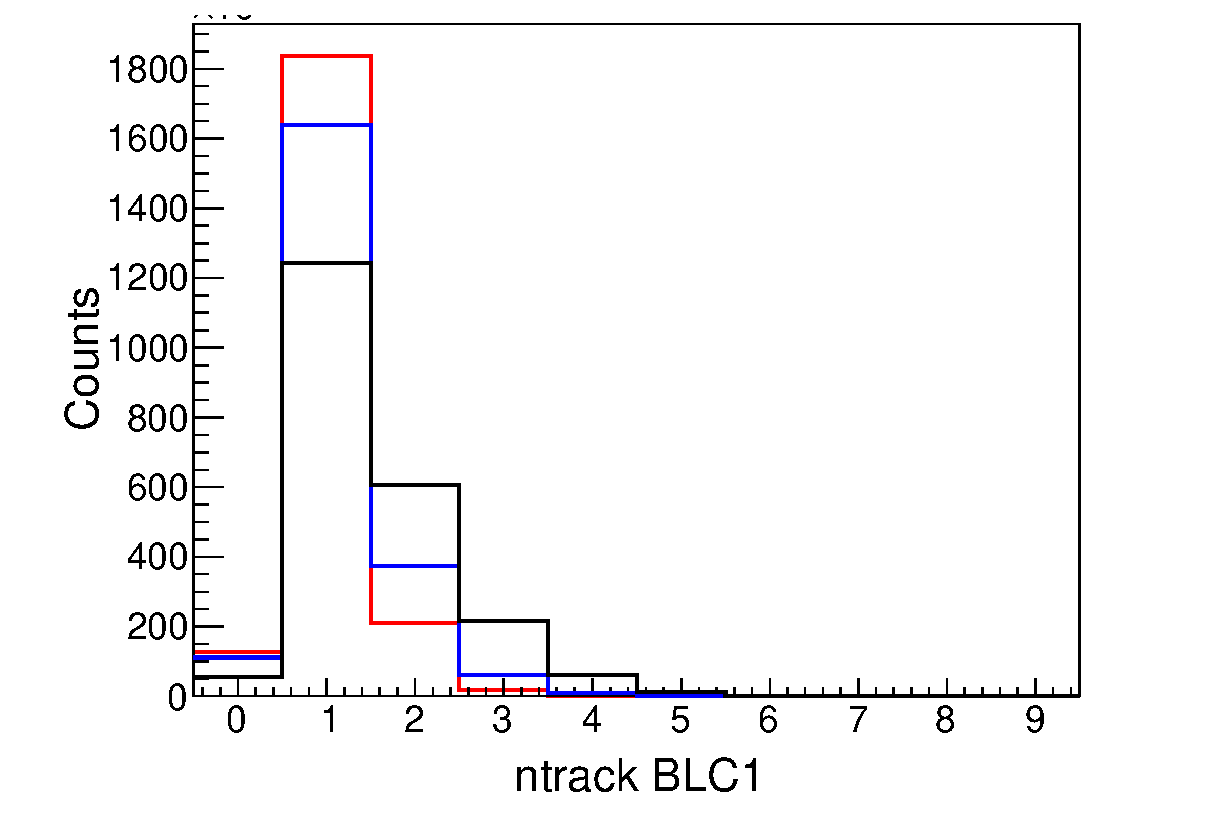
\includegraphics[width=4cm]{../pic/Run78/BL/nBLC1.eps}
    \end{minipage}
    \begin{minipage}{0.33\hsize}
      \includegraphics[width=4cm]{../pic/Run78/BL/BLC1_time.eps}
    \end{minipage}
    \begin{minipage}{0.33\hsize}
      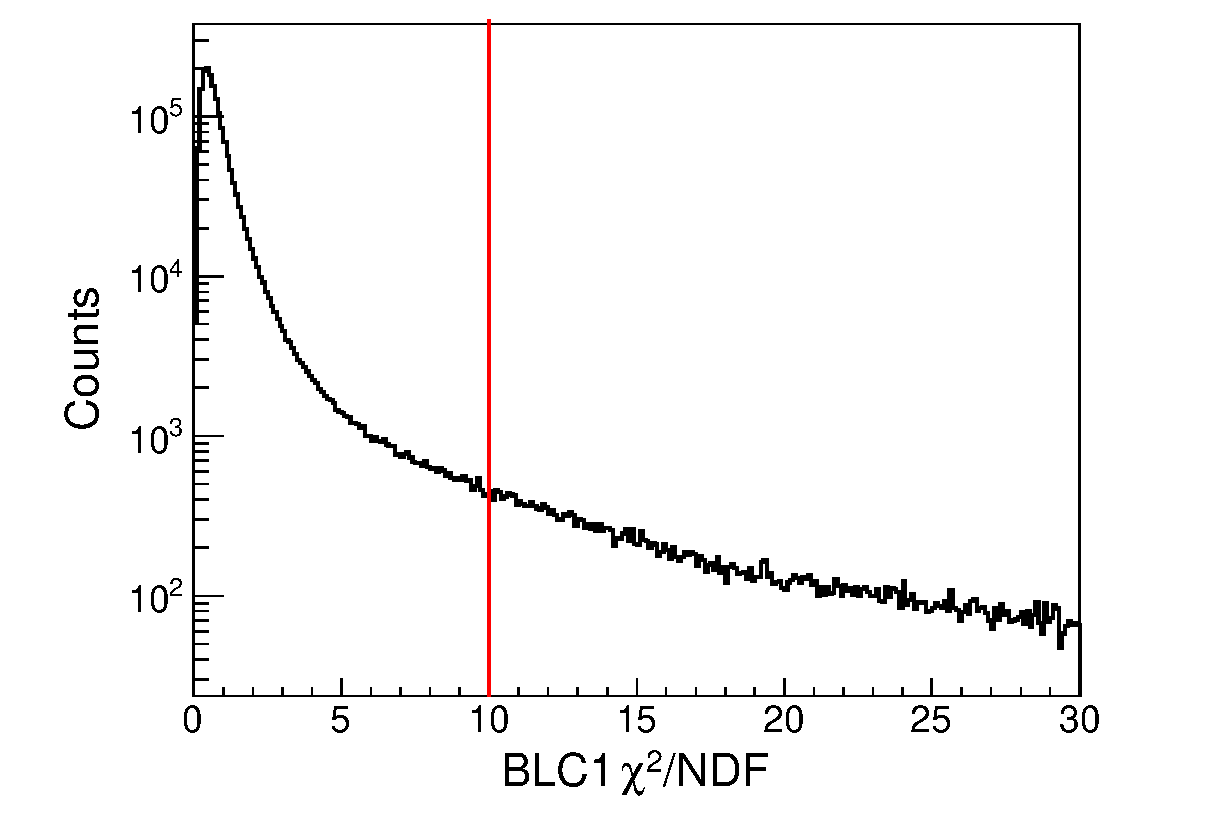
\includegraphics[width=4cm]{../pic/Run78/BL/BLC1_chi2.eps}
    \end{minipage}
  \end{tabular}
  
  \begin{tabular}{ccc}
    \begin{minipage}{0.33\hsize}
      \includegraphics[width=4cm]{../pic/Run78/BL/nBLC2.eps}
    \end{minipage}
    \begin{minipage}{0.33\hsize}
      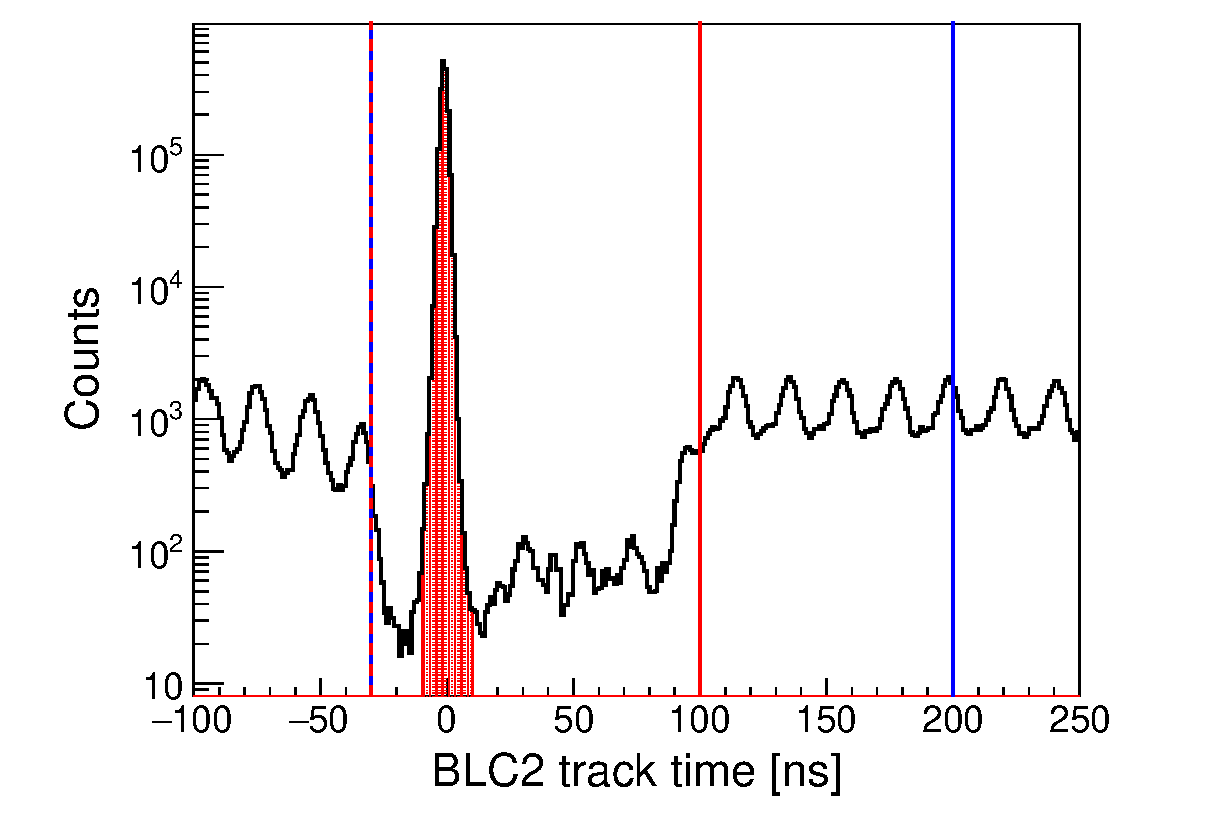
\includegraphics[width=4cm]{../pic/Run78/BL/BLC2_time.eps}
    \end{minipage}
    \begin{minipage}{0.33\hsize}
      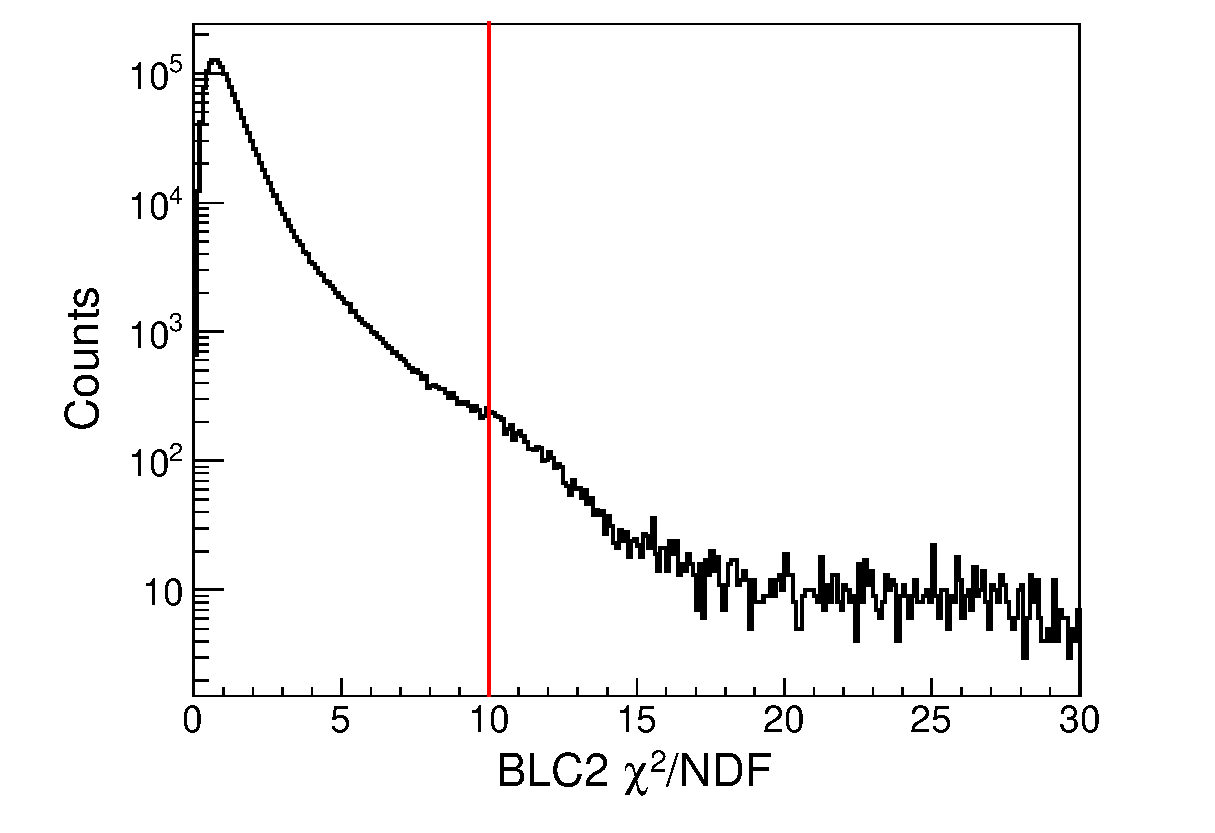
\includegraphics[width=4cm]{../pic/Run78/BL/BLC2_chi2.eps}
    \end{minipage}
  \end{tabular}
  
  \begin{tabular}{ccc}
    \begin{minipage}{0.33\hsize}
      \includegraphics[width=4cm]{../pic/Run78/BL/nBPC.eps}
    \end{minipage}
    \begin{minipage}{0.33\hsize}
      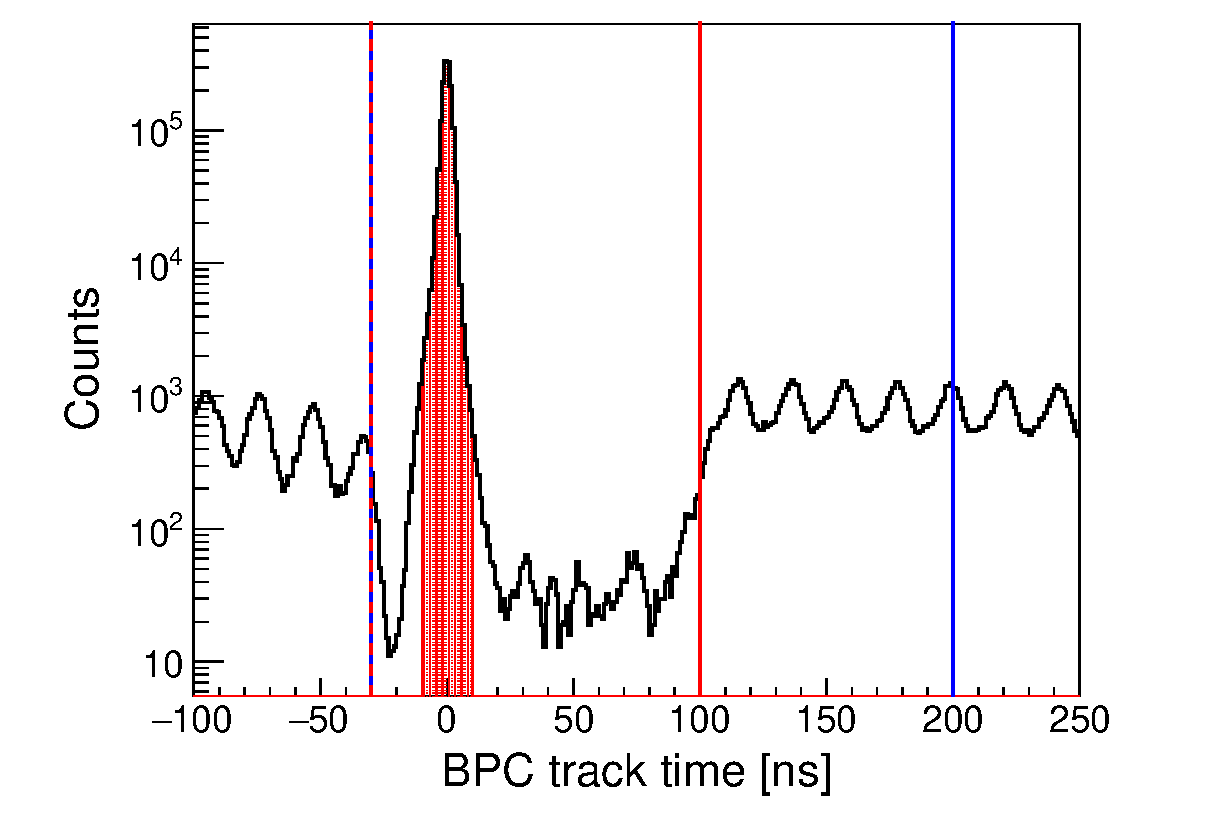
\includegraphics[width=4cm]{../pic/Run78/BL/BPC_time.eps}
    \end{minipage}
    \begin{minipage}{0.33\hsize}
      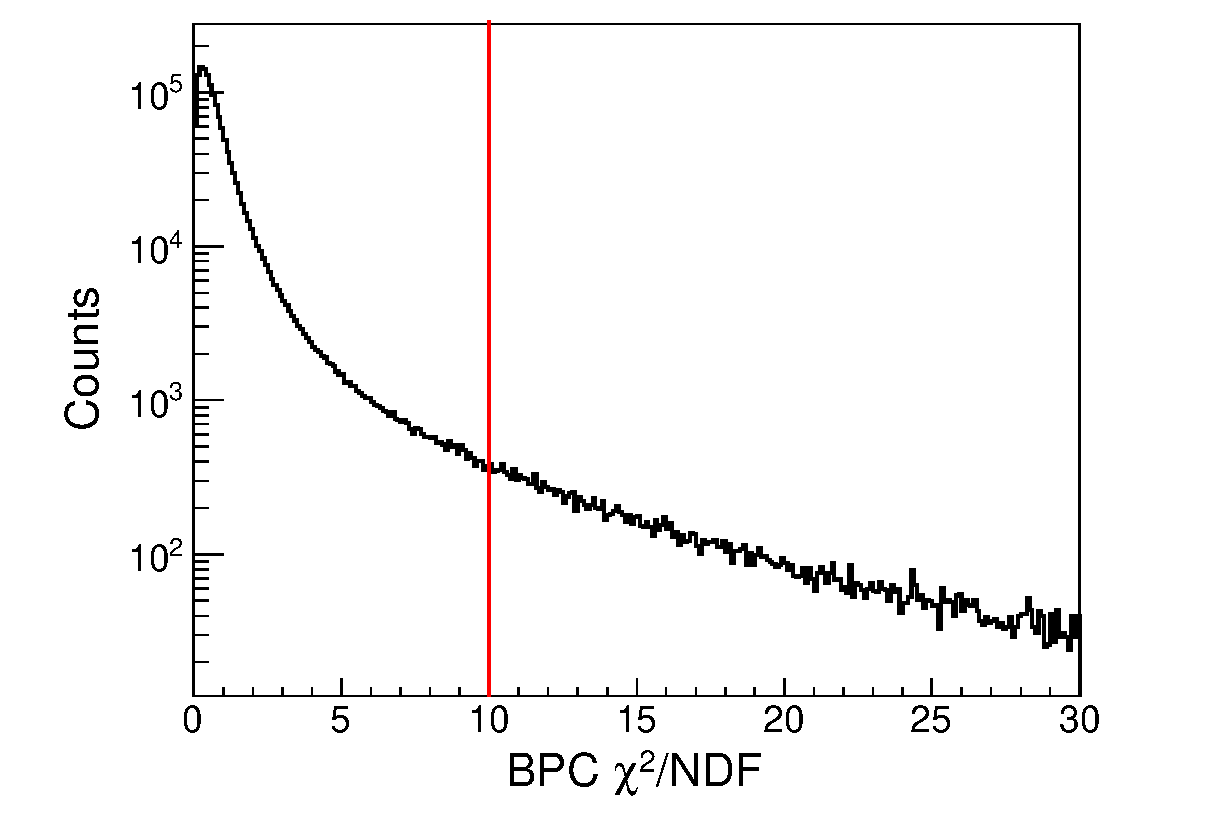
\includegraphics[width=4cm]{../pic/Run78/BL/BPC_chi2.eps}
    \end{minipage}
  \end{tabular}
  \caption{
    The left, the middle and the right figures show the number of tracks, track time and $\chi/NDF$, respectively.
    Color plots in the left figure indicate some time window.
    % Black, blue, red indicate all, $-30\sim200$[ns], $-30\sim100$[ns], respectively.
    The above, the middle and the down figures represent BLC1, BLC2 and BPC, respectively.
    The BPC was described after.
  }
  \label{fig:BLC_etc}
\end{figure}
BLC1 and BLC2 were installed upstream and downstream of the D5 magnet, respectively to measure beam momentum using the transfer matrix of the D5 magnet.
These are planer the type drift chamber whose drift length was calculated using the X-T map, which was the integration of drift time.
The track time of BLC was estimated from timing signals of pair plane due to constant drift length.
SX beam has RF-structure seems like the center figures of Fig\ref{fig:BLC_etc}, so we select synchronization about beam which indicates the red hatched region.
The left figures represent the number of tracks, in which black, blue, and red indicate time window of all, $-30\sim100$[ns], and $-30\sim200$[ns], respectively.
We select 1track events in red time window selection to keep statistics.
The right figures show $\chi^2/NDF$ distribution after 1track selection.
We accepted $\chi^2/NDF<10$ events as good track.



